\newchapter{Serwer}{Adrianna Piekarska}
\label{chap:server}

    Niniejszy rozdział przedstawia zagadnienia związane z procesem implementacji części serwerowej systemu. Uzasadnia wybór wykorzystanych technologii, prezentuje budowę i przepływ sterowania zarówno oprogramowania autoryzującego, jak i zarządzającego.

    Założeniem tej części procesu implementacyjnego nie było stworzenie skomplikowanego oprogramowania klasy biznesowej umożliwiającego zaawansowaną konfigurację systemu, lecz w pełni funkcjonalnego prototypu na potrzeby demonstracyjne. Wymienione technologie są wystarczające na potrzeby aplikacji prototypowych, jednak w przypadku chęci rozwijania systemu dla środowisk produkcyjnych konieczne mogłoby okazać się przemyślenie zestawu technologii w celu optymalizacji oraz zwiększenia bezpieczeństwa systemu.

    \section{Wykorzystane technologie}

    	\subsection{Linux Lubuntu}

    		Ze względu na wykorzystanie przenośnych technologii oprogramowanie serwera jest niezależne od systemu operacyjnego. W procesie implementacji i testowania systemu jako maszynę serwerową wykorzystano maszynę wirtualną z systemem Linux Lubuntu. Lubuntu jest szybkim i lekkim systemem operacyjnym bazującym na systemie Ubuntu i wykorzystującym minimalne środowisko graficzne LXQt (ang. \textit{The Lightweight Qt Desktop Environment}). Do wirtualizacji wykorzystano program VirtualBox.

    	
    	\subsection{Python}

    		Kluczową cechą na którą zwrócono uwagę przy wyborze technologii była możliwość szybkiego stworzenia prostej, funkcjonalnej aplikacji. Istotnym wymaganiem była także możliwość i wygoda przeprowadzania nieskomplikowanych operacji na bazie danych. Z tego powodu, do implementacji elementów serwera komunikujących się bezpośrednio z bazą danych wybrano język Python.

    		Python jest interpretowanym, przenośnym językiem programowania wysokiego poziomu o prostej i czytelnej składni oraz dynamicznym typowaniu. Wymienione cechy zmniejszają nakłady czasu związane z procesem wytwarzania i testowania rozwiązań w stosunku do języków kompilowanych.

    		Dzięki rozbudowanemu zestawowi bibliotek standardowych umożliwia łatwą integrację z bazą danych SQLite.  

    		Wykorzystano następujące biblioteki języka Python:

    		\begin{itemize}
    			\item \texttt{flask}

    			Jako język implementacji aplikacji API wchodzącej w skład oprogramowania zarządzajacego wybrano język Python z framework'iem Flask. Flask to lekka, popularna platforma do tworzenia aplikacji internetowych, zawierająca deweloperski serwer WWW. Cechuje się skalowalnością i elastycznością struktury i zależności projektu. 

    			\item \texttt{ssl}

    			W celu implementacji mechanizmu bezpiecznej komunikacji oprogramowania autoryzacji wykorzystana została wbudowana biblioteka \texttt{ssl}. Moduł ten zapewnia szereg funkcjonalności takich jak szyfrowanie oraz autoryzacja serwera i klienta. Do jego działania potrzebna jest biblioteka OpenSSL. 

    			\item \texttt{sqlite3}

    			Moduł \texttt{sqlite3} jest standardową biblioteką języka Python przeznaczoną do obsługi bazy danych SQLite. Moduł zapewnia interfejs SQL zgodny ze specyfikacją DB-API 2.0 zawartą w PEP 249.

    		\end{itemize}

    	\subsection{Angular}

    	    Istotnym czynnikiem motywującym wybór technologii była łatwość implementacji oraz rozwoju funkcjonalnej i estetycznej aplikacji demonstracyjnej, dlatego jako technologię implementacji aplikacji GUI zdecydowano się na framework Angular. Angular jest otwartą platformą do tworzenia tzw. SPA (ang. \textit{Single Page Applications}). SPA to aplikacje internetowe, w których nawigacja polega na dynamicznym ładowaniu poszczególnych elementów strony zamiast pobierania całych stron z serwera. Angular napisany jest w języku TypeScript, który jest otwartoźródłowym, typowanym nadzbiorem języka JavaScript. TypeScript jest również używany jako podstawowy język w projekcie Angular.

    	    Angular CLI jest narzędziem wspierającym pracę z framework'iem Angular poprzez udostępnienie zestawu prostych komend ułatwiających wykonywanie operacji związanych z procesem rozwijania aplikacji, takich jak tworzenie projektu, generowanie kodu źródłowego czy testowanie z użyciem wbudowanego serwera.

    	\subsection{SQLite}
    	\label{s:db}

    		Istotnym kryterium przydatności systemu zarządzania bazą danych była lekkość i łatwość obsługi z poziomu aplikacji internetowej napisanej w języku Python. Z tego względu zdecydowano się na system SQLite. Jest to prosty system zarządzania bazą danych, obsługujący język SQL (ang. \textit{Structured Query Language}), często stosowany w systemach wbudowanych. Nie wymaga instalacji odrębnego serwera. Posiada API do wielu języków programowania, w tym Pythona. Zawartość bazy danych przechowywana jest w pojedynczym pliku na dysku. Wszystkie powyższe cechy czynią SQLite rozwiązaniem przydatnym w szeroko pojętym procesie prototypowania.


    \section{Oprogramowanie autoryzujące}
    \label{s:auth_subs}

		Zadania należące do oprogramowania autoryzującego to komunikacja z układem zamka oraz interakcja z bazą danych. 
    	Oprogramowanie autoryzujące składa się z pojedynczego skryptu, którego działanie opiera się na cyklicznej obsłudze żądań urządzeń klienckich. Schemat blokowy oprogramowania autoryzującego przedstawia rysunek \ref{fig:flowchart5}.

    	\begin{figure}[]
            \centering
            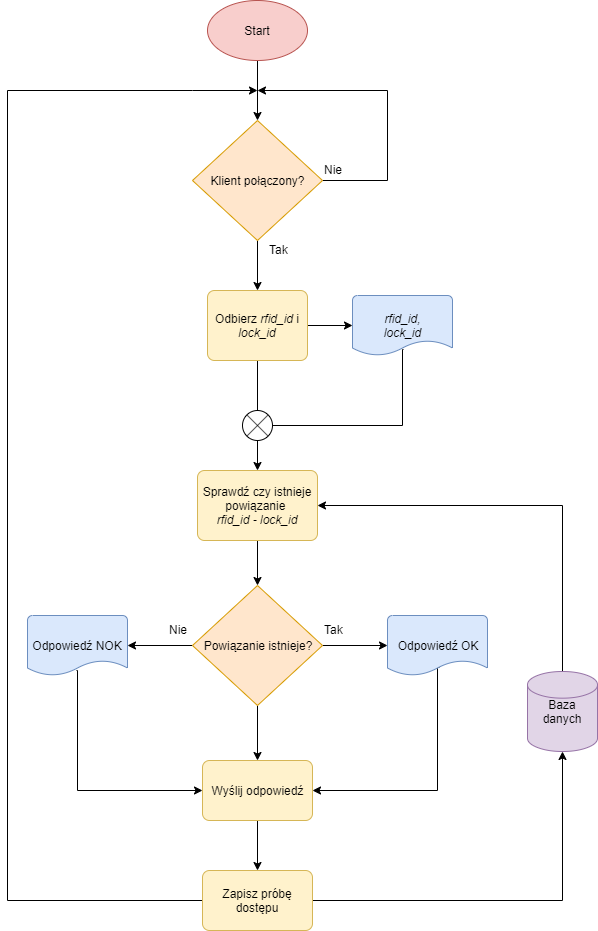
\includegraphics[width=0.85\textwidth]{chapters/images/flowchart5.png}
            \caption{Schemat blokowy przepływu sterowania oprogramowania autoryzującego}
            \label{fig:flowchart5}
        \end{figure}

    	W celu realizacji komunikacji z wykorzystaniem protokołu TLS użyto biblioteki \texttt{ssl} języka Python bazującej na OpenSSL. Uwierzytelnienie klienta zostało osiągnięte poprzez konfigurację kontekstu SSL w taki sposób, aby tryb weryfikacji wymagał poświadczenia tożsamości klienta w formie odpowiedniego certyfikatu.

    	Na potrzeby prototypu przyjęto, że baza danych i oprogramowanie autoryzujące znajdują się fizycznie na tej samej maszynie. Sprawia to, że oprogramowanie autoryzujące może w prosty sposób komunikować się z bazą danych zawartą w pliku znajdującym się na dysku. Fizyczne rozmieszczenie elementów przedstawia rysunek \ref{fig:fiz}.

    	\begin{figure}[]
            \centering
            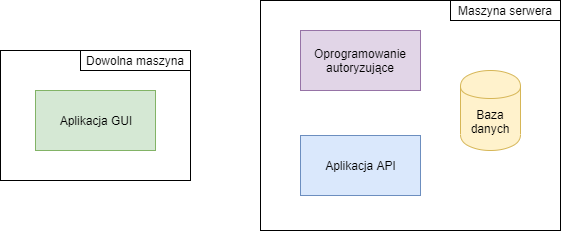
\includegraphics[width=\textwidth]{chapters/images/fiz.png}
            \caption{Fizyczne rozmieszczenie komponentów tworzących podsystemy autoryzacji i zarządzania}
            \label{fig:fiz}
        \end{figure}

    \section{Oprogramowanie zarządzające}

    	Oprogramowanie zarządzające zostało podzielone na dwie współpracujące ze sobą aplikacje. Warstwową budowę oprogramowania zarządzającego przedstawia rysunek \ref{fig:mngmt_subs_layers}. Wyodrębnienie aplikacji udostępniającej zasoby poprzez REST API (ang. \textit{Representational State Transfer API}) umożliwia rozszerzenie systemu o aplikacje klienckie przeznaczone na urządzenia mobilne. Również dzięki temu podziałowi możliwe jest fizyczne oddzielenie części GUI od maszyny, na której znajdują się oprogramowanie autoryzujące i aplikacja API.

        \begin{figure}[]
            \centering
            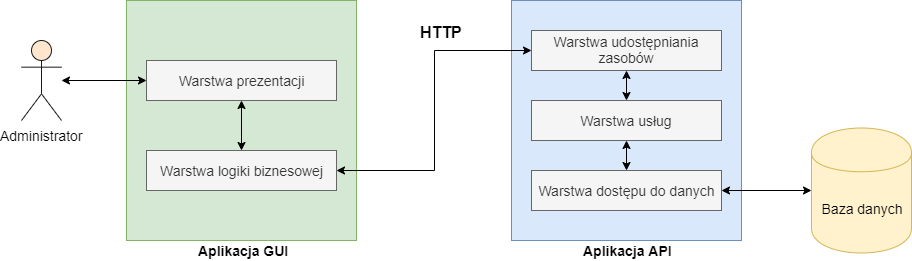
\includegraphics[width=\textwidth]{chapters/images/mngmt_subsystem_layers.png}
            \caption{Warstwowa budowa oprogramowania zarządzającego}
            \label{fig:mngmt_subs_layers}
        \end{figure}

    	\begin{itemize}
    		\item Aplikacja GUI (frontend)

				Aplikacja GUI jest interfejsem pomiędzy administratorem systemu a aplikacją API. Odpowiada za prezentację danych użytkownikowi, tłumaczenie jego akcji przeprowadzanych w środowisku graficznym na żądania HTTP i wysyłanie ich do aplikacji API.

				Zrzuty ekranu aplikacji GUI przedstawiono na rysunkach. Są to widok tabeli identyfikatorów RFID (\ref{fig:ss1}), widok okna dodawania nowego identyfikatora (\ref{fig:ss2}) oraz widok tabeli zawierającej historię prób dostępu (\ref{fig:ss3}).

				\begin{figure}[]
		            \centering
		            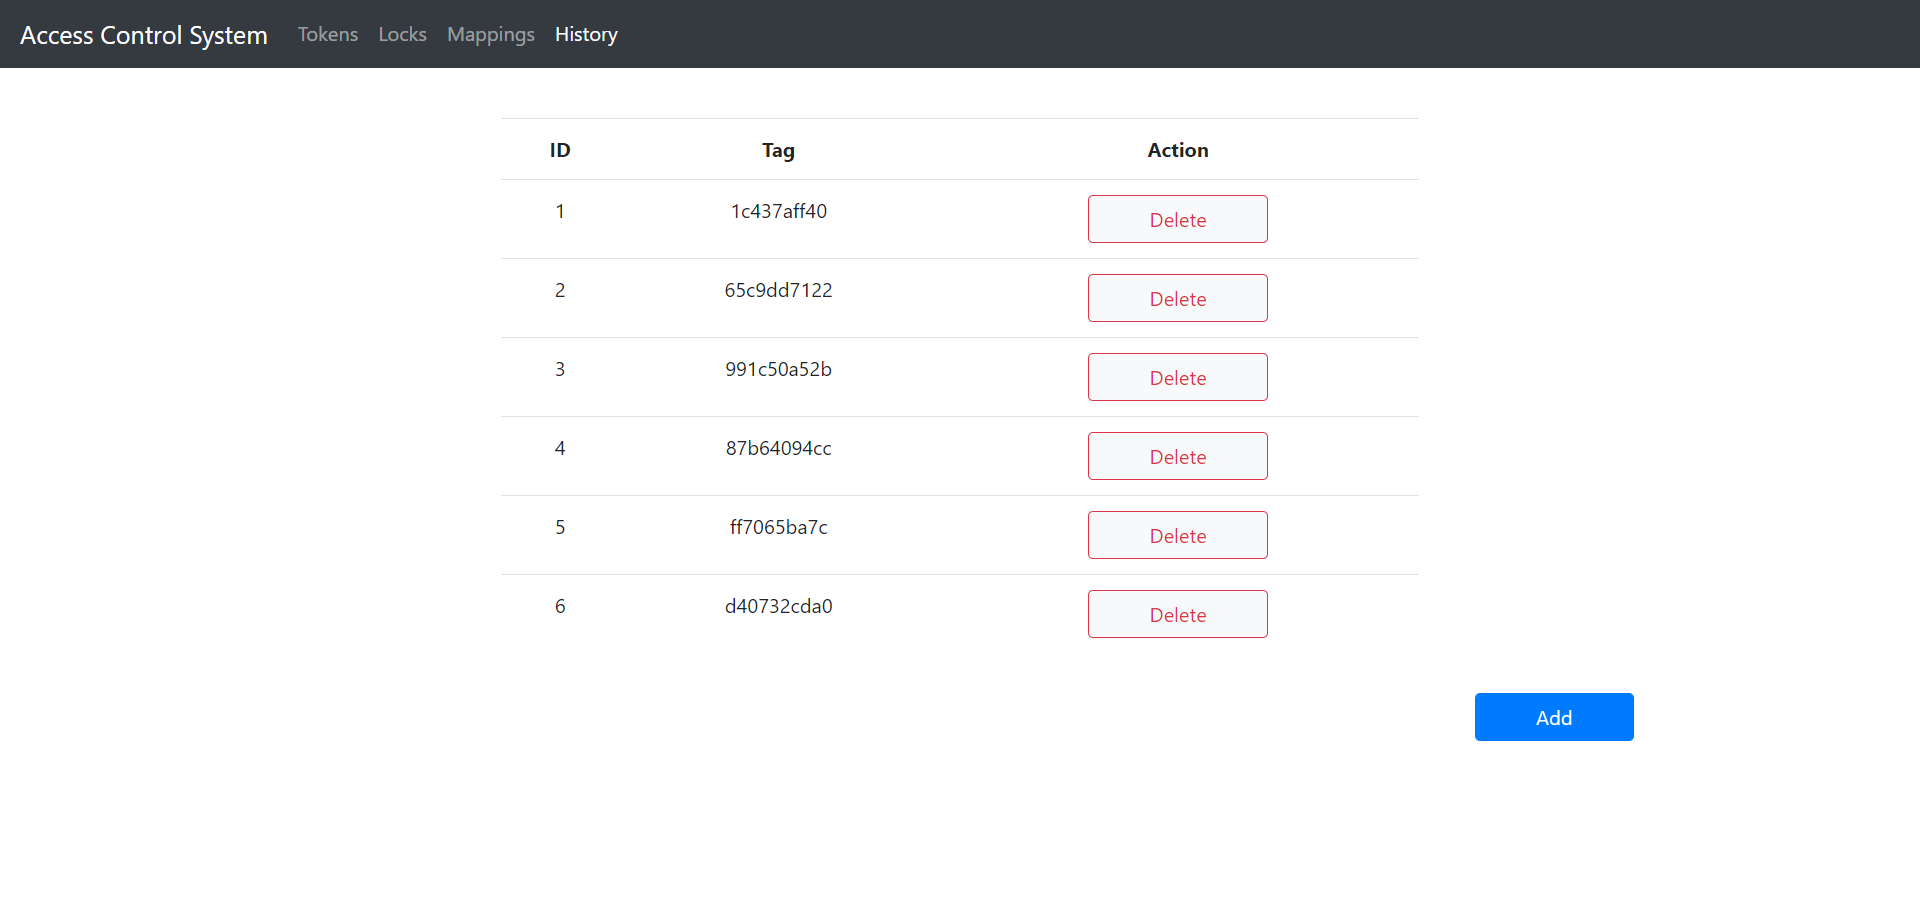
\includegraphics[width=\textwidth, frame]{chapters/images/ss1.png}
		            \caption{Zrzut ekranu widoku tabeli identyfikatorów RFID}
		            \label{fig:ss1}
		        \end{figure}

		        \begin{figure}[]
		            \centering
		            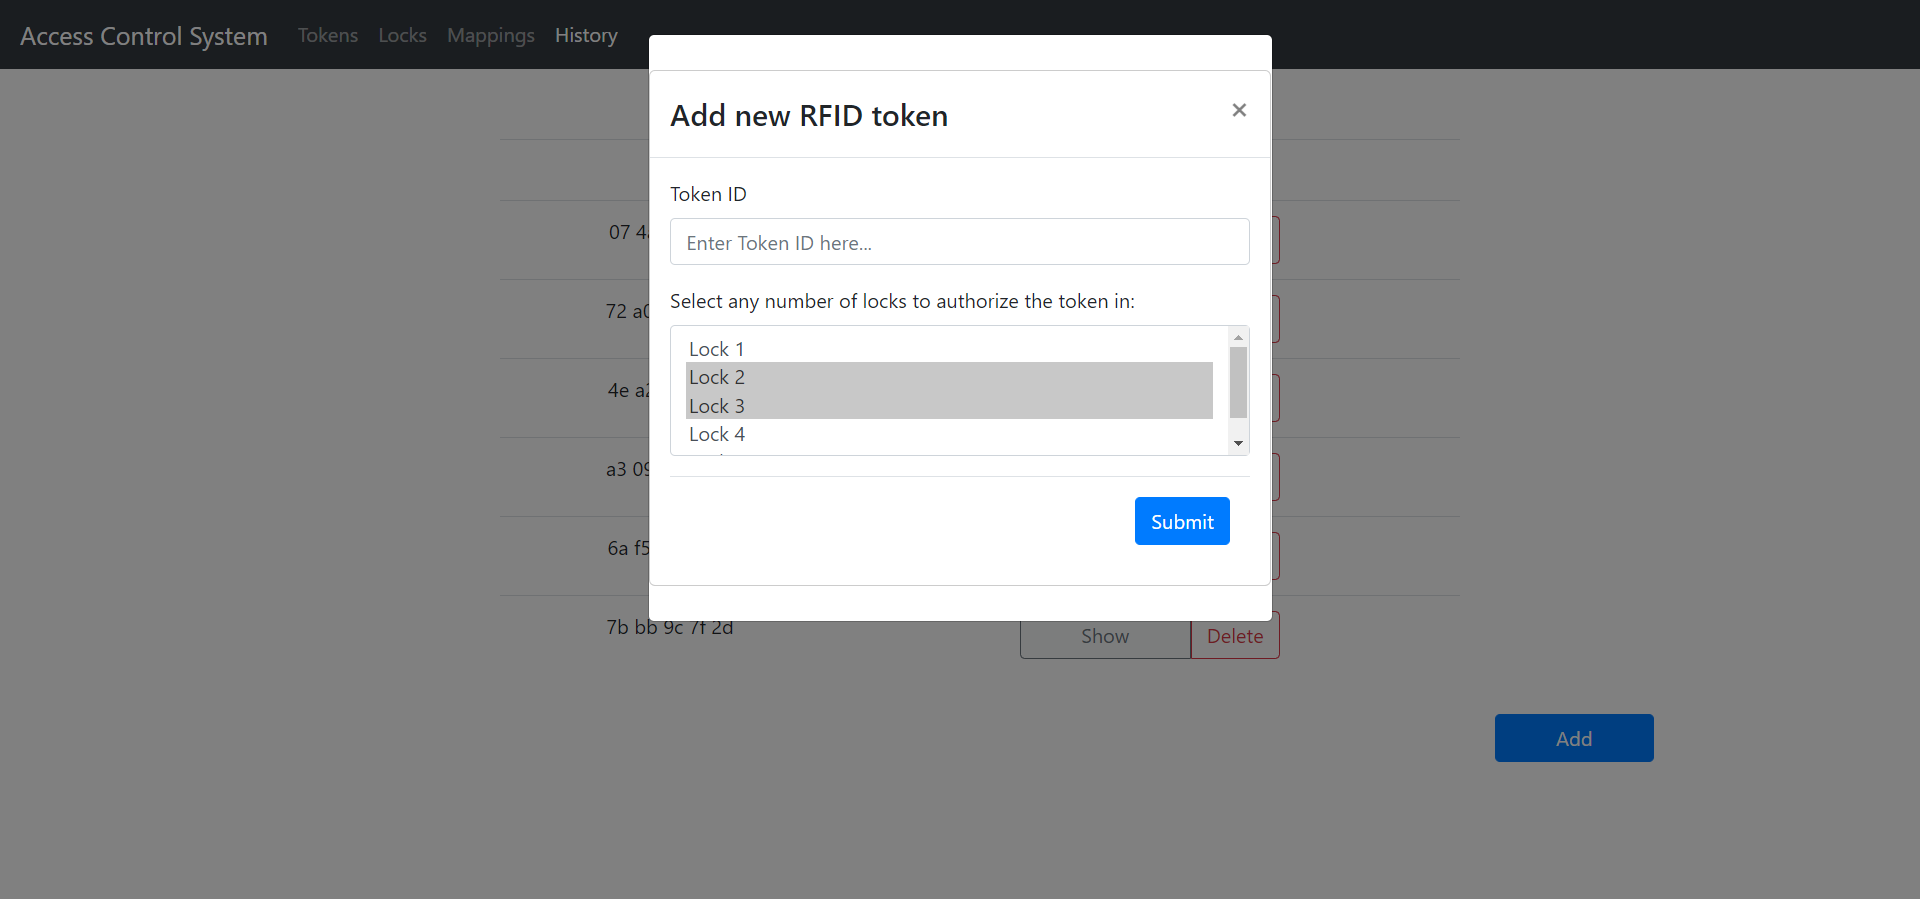
\includegraphics[width=\textwidth]{chapters/images/ss2.png}
		            \caption{Zrzut ekranu widoku okna dodawania nowego identyfikatora}
		            \label{fig:ss2}
		        \end{figure}

		        \begin{figure}[]
		            \centering
		            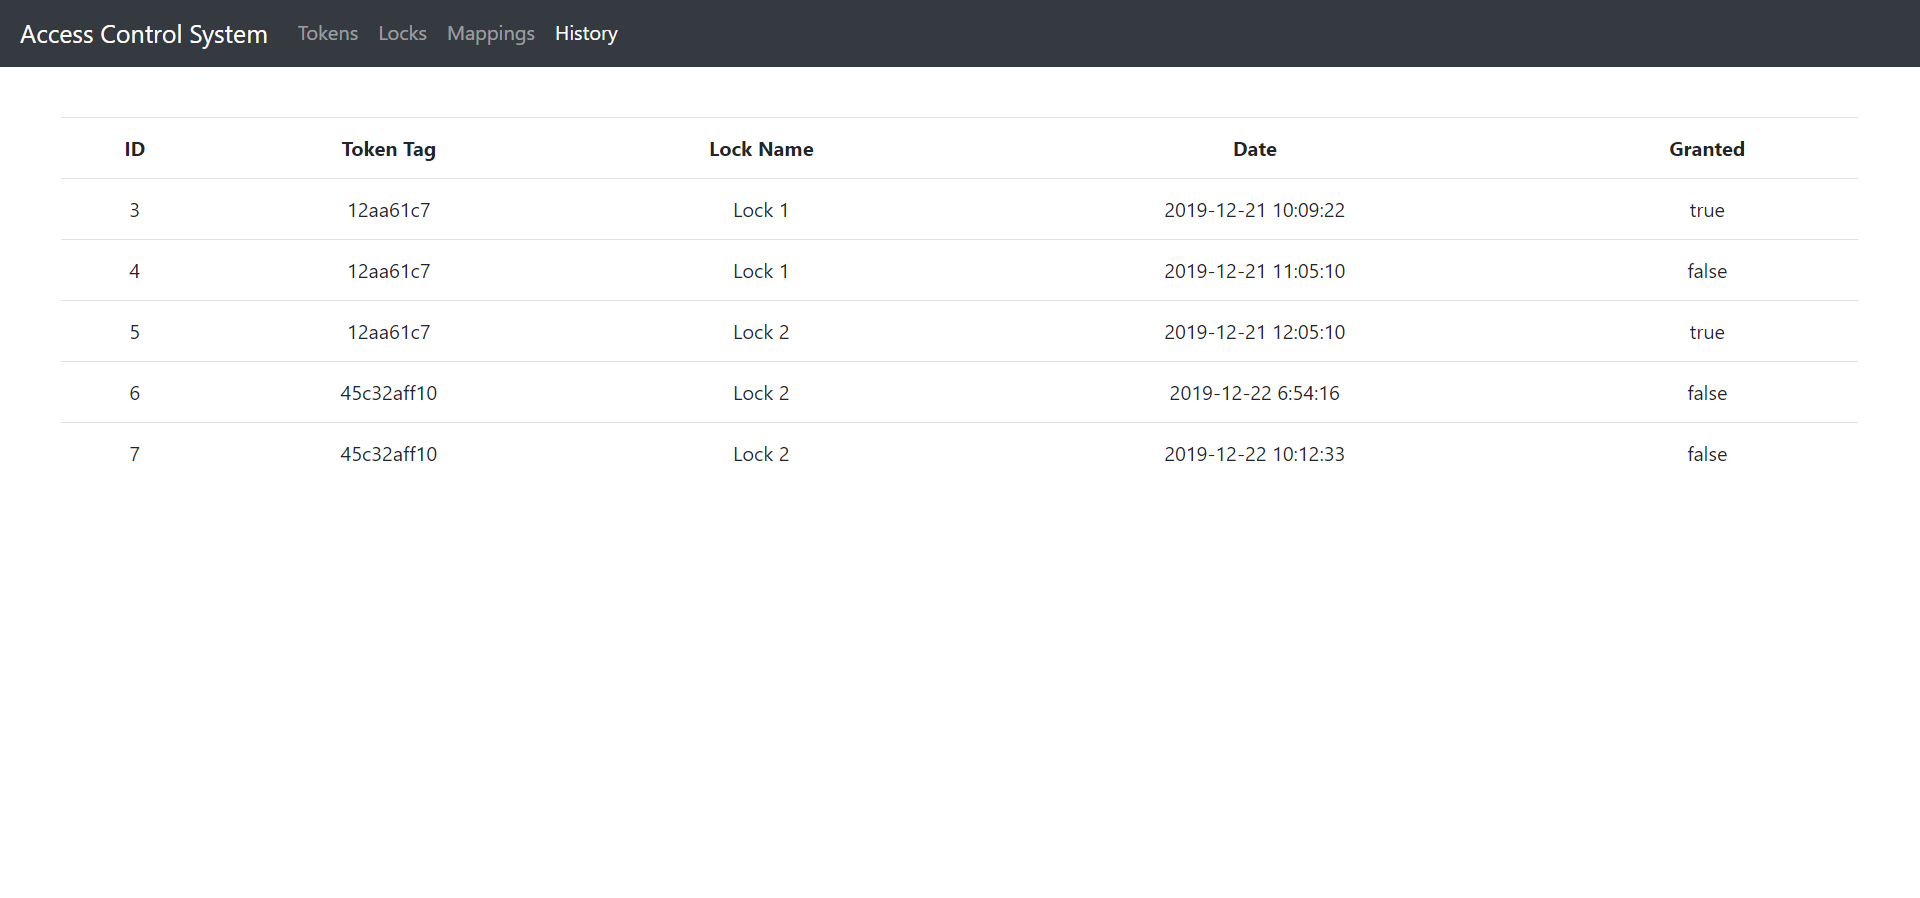
\includegraphics[width=\textwidth, frame]{chapters/images/ss3.png}
		            \caption{Zrzut ekranu widoku tabeli historii prób dostępu}
		            \label{fig:ss3}
		        \end{figure}

    		\item Aplikacja API (backend)

    			Aplikacja API udostępnia zasoby dla aplikacji GUI poprzez REST API. Odpowiada za odbieranie od niej żądań HTTP, przetwarzanie ich i zwracanie stosownych odpowiedzi. Zawiera logikę biznesową oraz logikę zarządzania i dostępu do danych. Składa się z warstwy definiującej punkty końcowe (ang. \textit{endpoints}), warstwy usług oraz warstwy dostępu do danych (modelu). Jej budowę przedstawiono na rysunku \ref{fig:api}.

				\begin{figure}[h!]
	            	\centering
		            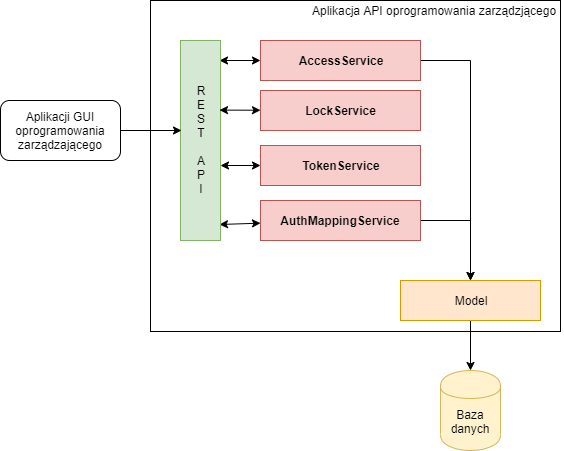
\includegraphics[width=\textwidth]{chapters/images/uslugi.png}
		            \caption{Budowa aplikacji API}
		            \label{fig:api}
		        \end{figure}

    	\end{itemize}

